\documentclass{article}

\usepackage[utf8]{inputenc}
\usepackage{hyperref}
\usepackage{natbib}
\usepackage{bibentry}
\usepackage{color}
\usepackage{graphicx}
\usepackage{float}

\nobibliography*

\title{A tutorial for metaOmic}
\author{}
\date{ }
 
 
\begin{document}
 
\maketitle
 
\tableofcontents
 
\section{Introduction}
 
MetaOmics is a GUI for meta-analysis implemented using R shiny.
Current version includes MetaQC for quality control, 
MetaDE for differential expression analysis,
MetaPath for pathway enrichment analysis,
MetaClust for sparse clustering analysis,
MetaPCA for principal component analysis,
MetaKTSP for classification analysis,
MetaDCN for differential co-expression network analysis,
MetaLA for liquid association analysis.

In this tutorial, 
we will go through installation and usage step by step using a real example.

The metaOmics suit software is publicly available at \url{https://github.com/metaOmic/metaOmics}.
Individual R packages are also available on GitHub and the url will be introduced in each individual package section.

 
\section{Preliminaries}
\subsection{Citing MetaOmics}
MetaOmics software suite implements many meta-analysis methods from different authors. 
Please cite appropriate papers if you use MetaOmics,
by which the authors will receive professional credits for their work.

\begin{itemize}

\item MetaOmics software suite itself can be cited as: 

\begin{itemize}
\item Ma, T., Huo, Z., Kuo, A., Zhu, L., Fang, Z., Zeng, X., Lin, C.-W., Liu, S., Wang, L., Rahman, T., Chang, L.-C., Kim, S., Li, J., Park, Y., Song, C., Oesterreich, S., Sibille, E. and Tseng, G. C. MetaOmics: Comprehensive Analysis Pipeline and Browser-based Software Suite for Transcriptomic Meta-Analysis.
\end{itemize}

\item Review, comparative papers and published R packages:
\begin{itemize}
\item \bibentry{tseng2012comprehensive}.
\item \bibentry{chang2013meta}.
\item \bibentry{wang2012r}.
\end{itemize}

\item MetaQC: 
\begin{itemize}
\item (MetaQC) \bibentry{kang2012metaqc}.
\end{itemize}

\item MetaDE: 
\begin{itemize}
\item (Fisher) \bibentry{fisher1925statistical}.
\item (AW-Fisher) \bibentry{li2011adaptively}.
\item (AW-Fisher) \bibentry{huo2017p}.
\item (REM/FEM) \bibentry{choi2003combining}.
\item (rOP) \bibentry{song2014hypothesis}.
\item (minMCC) \bibentry{lu2009biomarker}.
\item (Stouffer) \bibentry{stouffer1949american}
\item (RankProd) \bibentry{hong2006rankprod} 
\end{itemize}

\item MetaPath: 
\begin{itemize}
\item (MAPE) \bibentry{shen2010meta}.
\item (CPI) \bibentry{fang2016cpi}.
\end{itemize}

\item MetaNetwork: 
\begin{itemize}
\item (MetaDCN) \bibentry{zhu2016metadcn}.
\end{itemize}

\item MetaPredict: 
\begin{itemize}
\item (MetaKTSP) \bibentry{Kim2016}.
\end{itemize}

\item MetaClust: 
\begin{itemize}
\item (MetaSparseKmeans) \bibentry{huo2016meta}.
\end{itemize}

\item MetaPCA: 

\begin{itemize}
\item (MetaPCA) \bibentry{kim2017meta}.
\end{itemize}

\end{itemize}



\subsection{How to start MetaOmics}

The full instruction of how to install and start MetaOmics software suite is also available at \url{https://github.com/metaOmics/metaOmics}.


\subsubsection{Requirement}
\begin{itemize}
\item R $>=$ 3.3.1
\item Shiny $>=$ 0.13.2
\end{itemize}



{\bf Note:}
\begin{itemize}
\item We recommend users to use R 3.3 to implement our tool. If you are using R 3.4 (released on 4/24/2017), you may encounter errors in installing dependencies of the modules. You can manually install the dependencies by running the following commands in R:

\textit{install.packages(c(\textquotesingle GSA\textquotesingle, \textquotesingle combinat\textquotesingle, \textquotesingle   samr\textquotesingle   , \textquotesingle   survival\textquotesingle   , \textquotesingle   cluster\textquotesingle   , \textquotesingle   gplots\textquotesingle   , 
  \textquotesingle   ggplot2\textquotesingle   , \textquotesingle   irr\textquotesingle   , \textquotesingle   shape\textquotesingle   , \textquotesingle   snow\textquotesingle   , \textquotesingle   snowfall\textquotesingle   , \textquotesingle   igraph\textquotesingle   , \textquotesingle   doMC\textquotesingle   , \textquotesingle   PMA\textquotesingle   ))
  }

\textit{source(\textquotesingle   https://bioconductor.org/biocLite.R\textquotesingle   )  }

\textit{biocLite(c(\textquotesingle   multtest\textquotesingle   , \textquotesingle   Biobase\textquotesingle   , \textquotesingle   edgeR\textquotesingle   , \textquotesingle   DESeq2\textquotesingle   , \textquotesingle   impute\textquotesingle   , 
  \textquotesingle   limma\textquotesingle   , \textquotesingle   AnnotationDbi\textquotesingle   , \textquotesingle   ConsensusClusterPlus\textquotesingle   , \textquotesingle   genefilter\textquotesingle   , \textquotesingle   GSEABase\textquotesingle   , \textquotesingle   Rgraphviz\textquotesingle   ))
  }

\item For Windows, users need to run the following command in R to install the package \textquotesingle doMC\textquotesingle:

\textit{install.packages(\textquotesingle doMC\textquotesingle, repos=\textquotesingle http://R-Forge.R-project.org\textquotesingle)}

\end{itemize}

 

\subsubsection{How to install the software}
\begin{itemize}
\item At MetaOmics home page \url{https://github.com/metaOmics/metaOmics}, clone the project by
clicking on ``Clone or download" and extract to a working directory, 
or type in the following in command line:

\textit{git clone} \url{https://github.com/metaOmic/metaOmics}
\end{itemize}

\subsubsection{How to start the software}
\begin{itemize}
\item Run from docker image.

\begin{enumerate}
\item Install docker (if not installed).
\item In terminal

\textit{docker pull metaomics/app}

\textit{docker run --rm --name metaOmics -p 3838:3838 metaomics/app}

\end{enumerate}


\item Run from R.

\begin{enumerate}
\item Open R 
\item Set the working directory such that metaOmics folder included. 

\textit{install.packages(\textquotesingle shiny\textquotesingle)}

\textit{shiny::runApp(\textquotesingle metaOmics\textquotesingle, port=9987, launch.browser=T)}
\end{enumerate}



\end{itemize}

\subsection{MetaOmics setting page}
\label{sec:setting}
After starting MetaOmics, 
the first page is the MetaOmics setting page as shown in Figure~\ref{fig:GUIsetting}.  
There are four tabs on the top of the page (See Figure~\ref{fig:GUIsetting} {\color{red} (1)}), 
which will direct users to specific functional modules of the software including Setting, Preprocessing, Saved Data and Toolsets.
Below these tabs is a {\bf Welcome to MetaOmics} section, which briefly introduce the software and other information about the authors and maintainers.
Further below, there are two sections: Session Information and Directory for Saving Output Files (See Figure~\ref{fig:GUIsetting} {\color{red} (2)}).
By clicking ``$\ldots$",
users can set working directory, in which all the meta-analysis results will be saved.
The current working directory is displayed on the top right corner (See Figure~\ref{fig:GUIsetting} {\color{red} (3)}).
There is one more section with the header Toolsets (See Figure~\ref{fig:GUIsetting} {\color{red} (4)}),
where users can click the blue button to install the desired modules if the ``Status" shows ``not installed".
If the packages are already installed, an icon of ``checked installed" will show up in ``Status".
%Otherwise, users can install individual package by clicking install blue button.
The installation progress may take up to a few minutes for each module.
A notification icon will pop up at the bottom right corner upon finishing the installation process. 
After the modules are installed, restart the MetaOmics software suite so that the Shiny application interface is updated with the installed modules.
(See Figure~\ref{fig:GUIsetting} {\color{red} (5)}) shows the current active dataset, 
which is introduced in Section~\ref{sec:procedure}~\ref{sec:active}. 
 
\begin{figure}[H]
\begin{center}
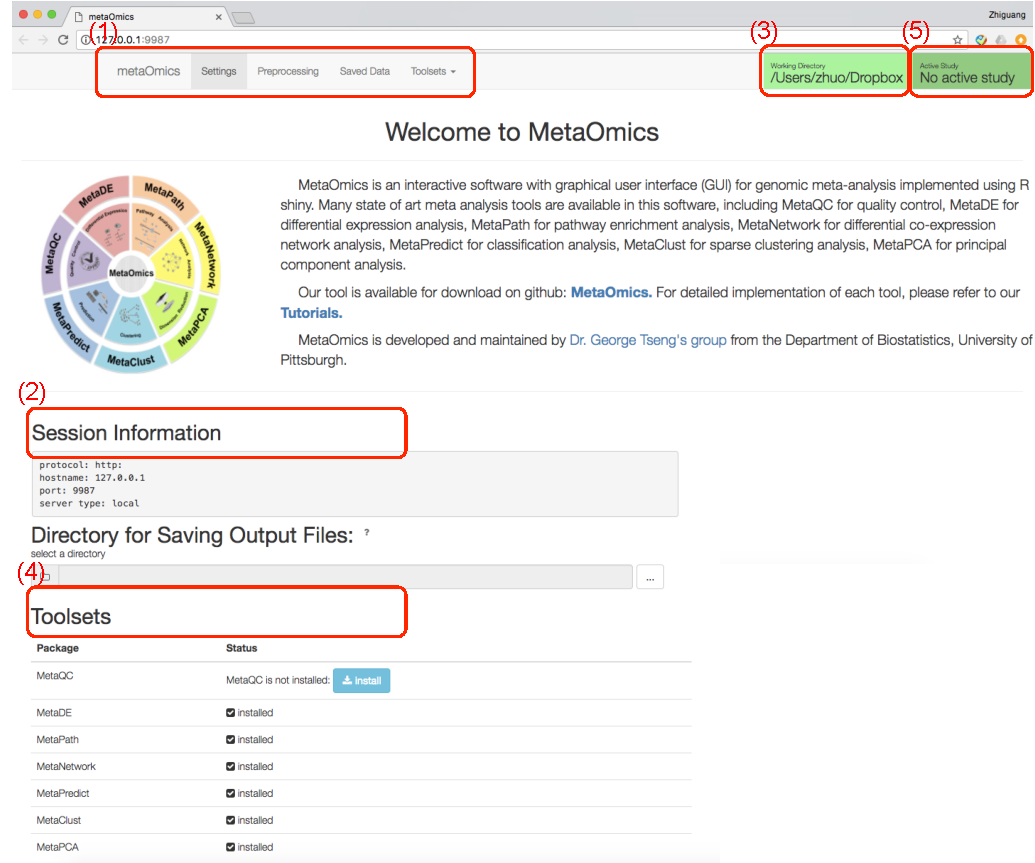
\includegraphics[scale=0.9]{./figure/preprocessing/GUIsetting}
\caption{MetaOmics software suite GUI setting page}
\label{fig:GUIsetting}
\end{center}
\end{figure}


\subsection{Question and bug report}

If you encounter errors or bugs, please report to maintainer Tianzhou Ma $<$\url{tim28@pitt.edu}$>$.


 
 
 
 
\section{Prepare data}
\label{sec:dataPrepare}
\subsection{Raw data}

Data should be prepared as the example in Figure~\ref{fig:dataMicroarray}.
First column should be feature ID (e.g. gene symbol) and the rest of the columns are samples.
The first row is sample ID.
Valid data type includes continuous, count.

\begin{figure}[H]
\begin{center}
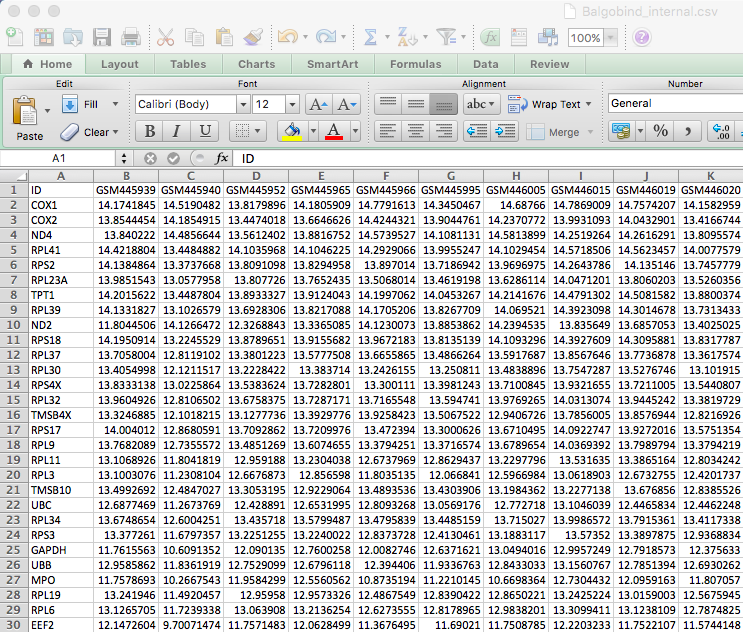
\includegraphics[scale=0.5]{./figure/dataMicroarray}
\caption{A example data format}
\label{fig:dataMicroarray}
\end{center}
\end{figure}

\subsection{Clinical data}

Clinical data should be prepared as the example in Figure~\ref{fig:clinical}.
First column should be sample ID and each row represents a sample.
The rest of the columns are clinical information.

\begin{figure}[H]
\begin{center}
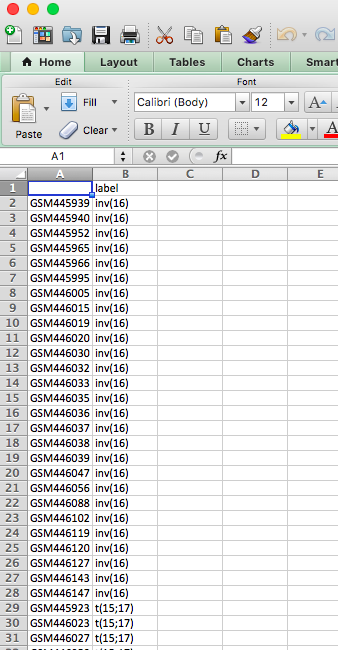
\includegraphics[scale=0.5]{./figure/clinicalData}
\caption{A example clinical data format}
\label{fig:clinical}
\end{center}
\end{figure}

\section{MetaOmics suit GUI}
\subsection{Setting}

After starting metaOmics, 
the first page is the metaOmics setting page in Figure~\ref{fig:GUIsetting}.  
There are 4 tabs on top of the page: Setting, Preprocessing, Saved Data and Toolsets.
Below the 4 tabs, 
the first header is the session information.
{
\color{red}
Why do we need session information?
}
The second header is Directory for Saving Output Files.
By clicking $\ldots$,
user can set default working directory, in which all the meta-analysis results will be saved.
User can view their current working directory on the top right corner.
The third header is Toolsets,
here users can view if individual packages are installed.
If the packages are installed, there is a checked installed status.
Otherwise, users can install individual package by clicking install blue button.

\begin{figure}[H]
\begin{center}
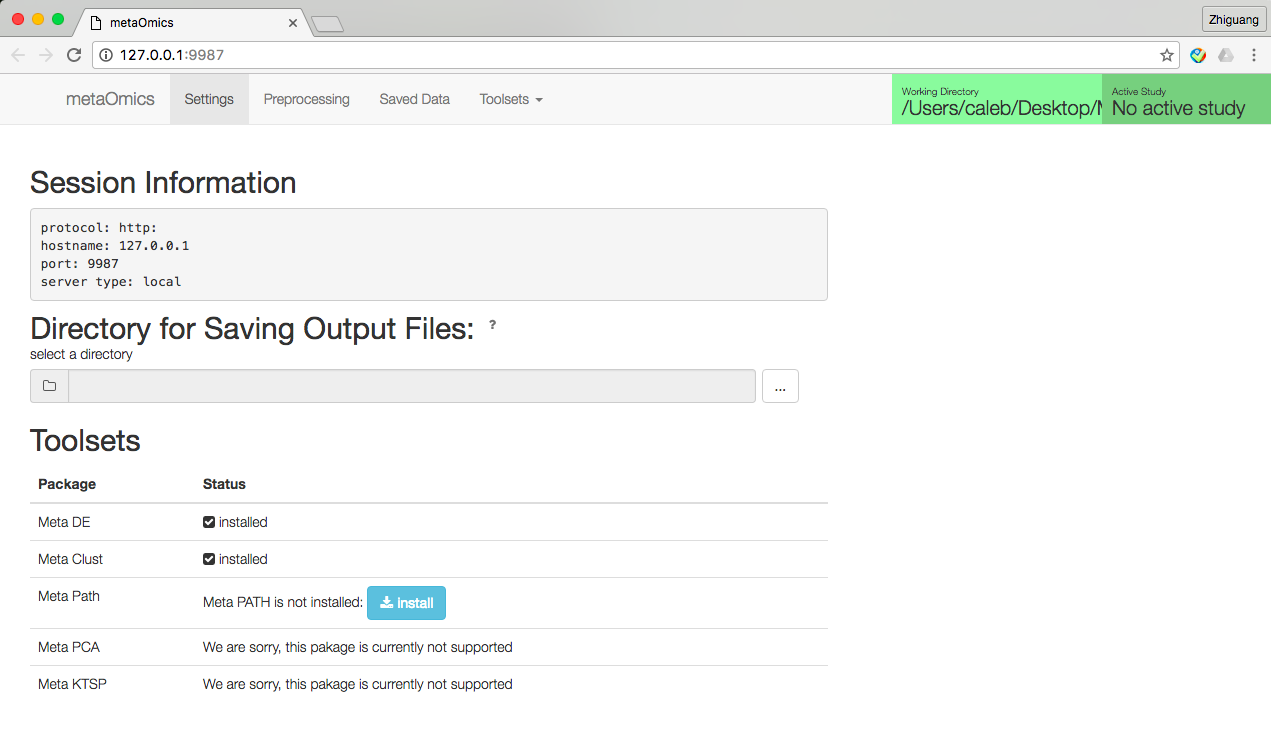
\includegraphics[scale=0.35]{./figure/GUIsetting}
\caption{GUI setting page}
\label{fig:GUIsetting}
\end{center}
\end{figure}

\subsection{Preprocessing}
If users go to the Preprocessing page as Figure~\ref{fig:GUIpreprocessing},
\begin{figure}[!htbp]
\begin{center}
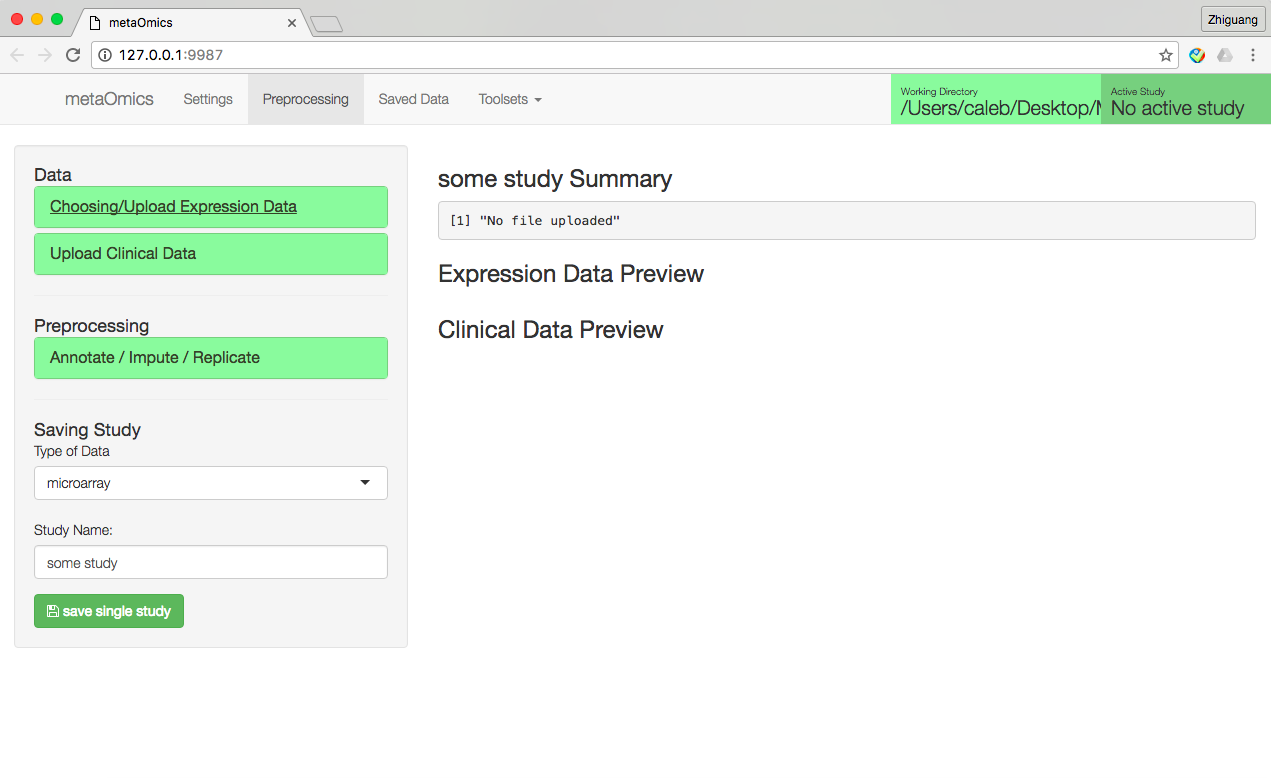
\includegraphics[scale=0.35]{./figure/GUIpreprocessing}
\caption{GUI Preprocessing page}
\label{fig:GUIpreprocessing}
\end{center}
\end{figure}
they are able to uploaded genomic data via the tab ``Choosing/Upload Expression Data".
The data should be prepared according to Section~\ref{sec:dataPrepare}.
Users may optionally upload Clinical Data, depending on purpose.
{
\color{red}
Check data requirement table?.
}
After uploading is complete,
users can preview their data on the right hand side of the page as Figure~\ref{fig:GUIpreview}.
There are several Expression Data Parsing Option available on the left panel.
\begin{figure}[H]
\begin{center}
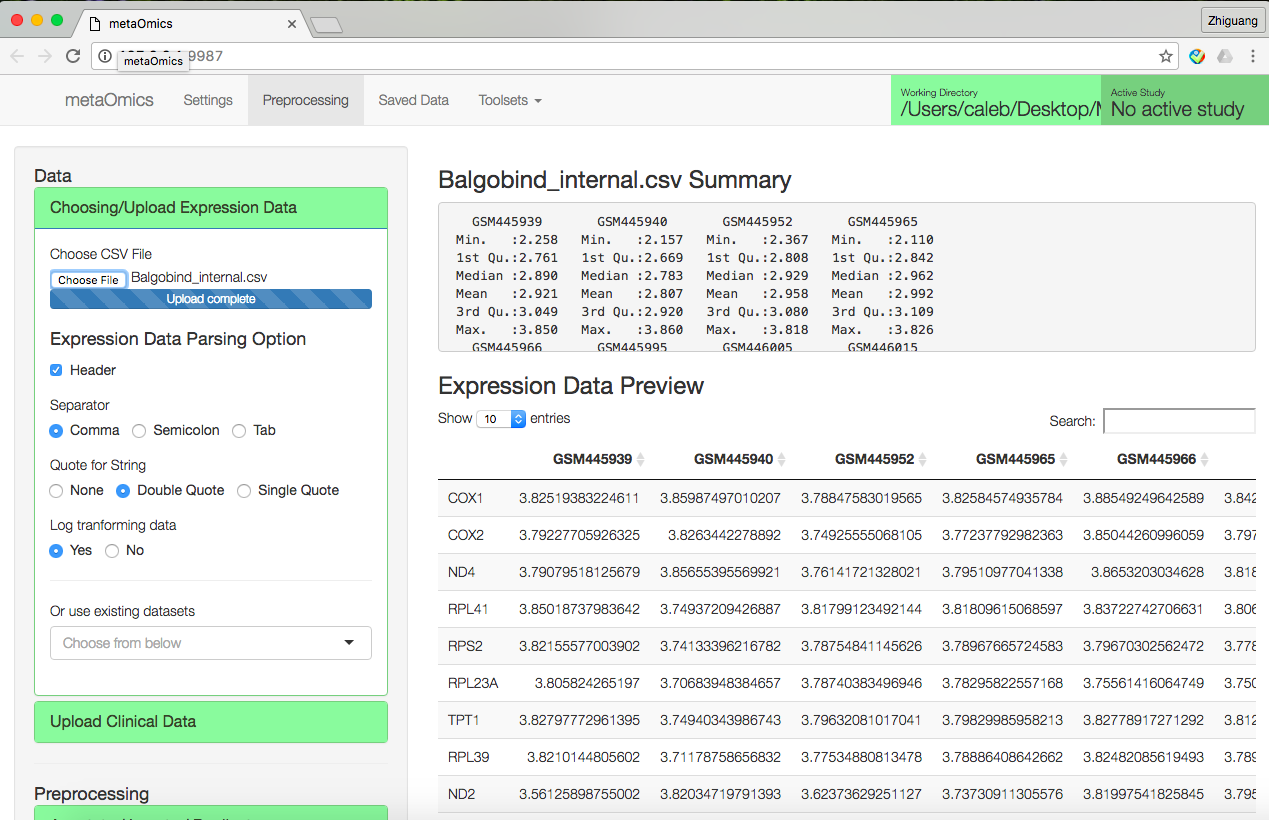
\includegraphics[scale=0.35]{./figure/GUIpreview}
\caption{GUI Preprocessing page}
\label{fig:GUIpreview}
\end{center}
\end{figure}
The MetaOmics suit also provide handlers for feature annotation, missing value imputation and multiple probe same genes.
Then users could specify type of data and study name.
Then click ``save single study" button, single study will be saved.

\subsection{Saved Data}
After uploading multiple studies w/o clinical data,
Users can turn to the Saved Data tab.
Users should select multiple datasets as Figure~\ref{fig:GUImerge}.
\begin{figure}[H]
\begin{center}
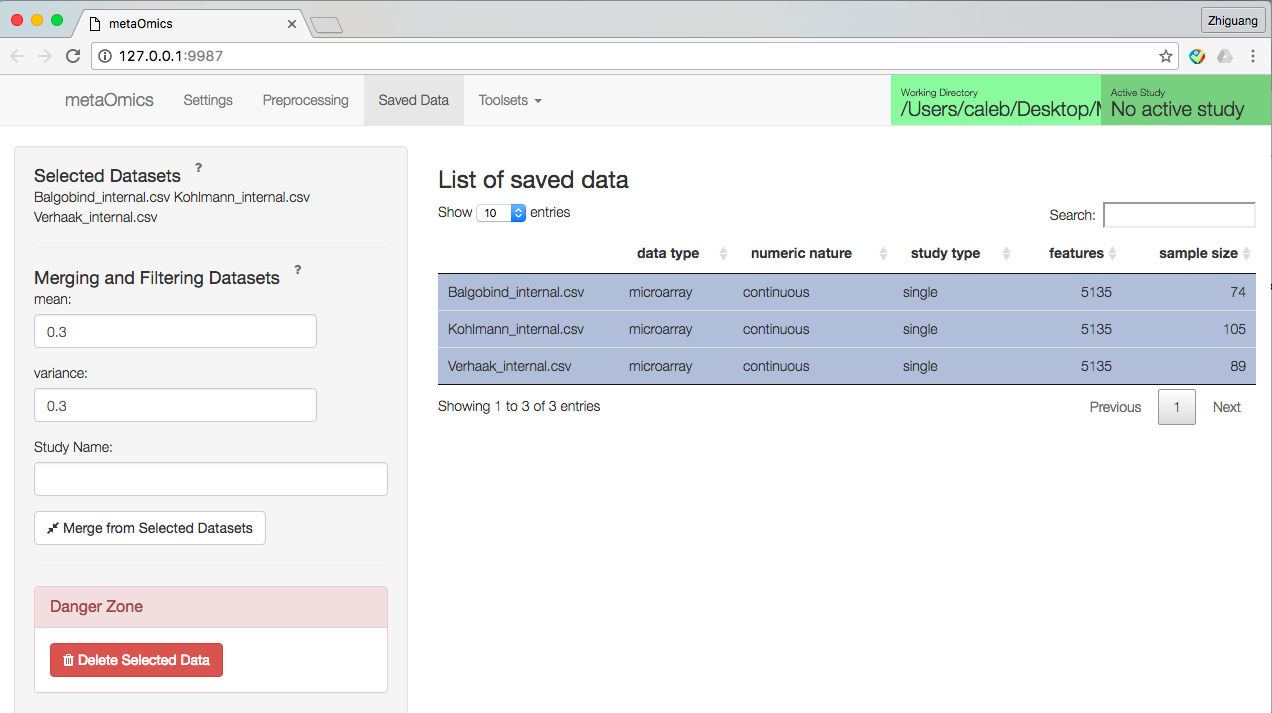
\includegraphics[scale=0.35]{./figure/GUImerge}
\caption{GUI Preprocessing page}
\label{fig:GUImerge}
\end{center}
\end{figure}
Users can select filtering criteria, enter merged study name and click on the Merge from Selected Datasets.
A merged dataset will appear on the left ``List of saved data" panel.
The last thing users need to do before using meta-analytic toolsets is select merged data and click on 
``Make merged Active Dataset" - A big green button.
Then the merged data becomes active study and shows up on the top right corner.

\section{Toolsets}


\subsection{MetaQC}

\subsection{MetaDE}

\subsection{MetaPath}

\subsection{MetaClust}
By clicking toolsets and then metaClust,
users are directed to metaClust home page as Figure~\ref{fig:metaClustHome}.
\begin{figure}[H]
\begin{center}
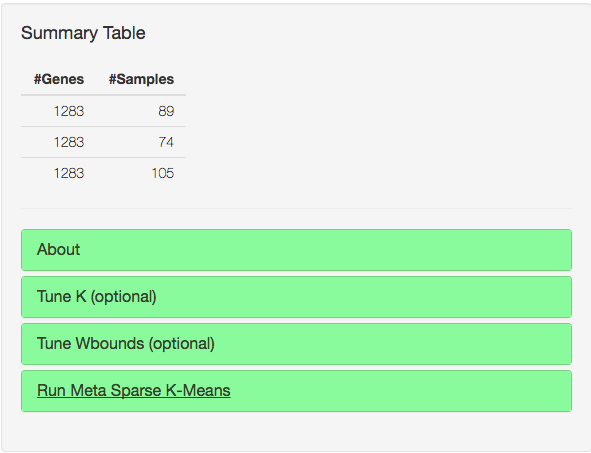
\includegraphics[scale=0.35]{./figure/metaClust/metaClustHome}
\caption{GUI Preprocessing page}
\label{fig:metaClustHome}
\end{center}
\end{figure}
On the top left panel users can see data summary Table.
Below there are 4 tabs.
\subsubsection{About}
About tab includes basic introduction of metaClust.
Starting with multiple studies, 
we could run MetaSparseKmeans with pre-specified number of clusters (K) and gene selection tuning parameter (Wbounds).
If you are not sure about what are good K and Wbounds, please try Tune K and Tune Wbounds panel.

\subsubsection{Tune K}
If the users are not sure what is number of clusters,
they can start to use the Tune K panel as in Figure~\ref{fig:metaClusttuneK}.
\begin{figure}[H]
\begin{center}
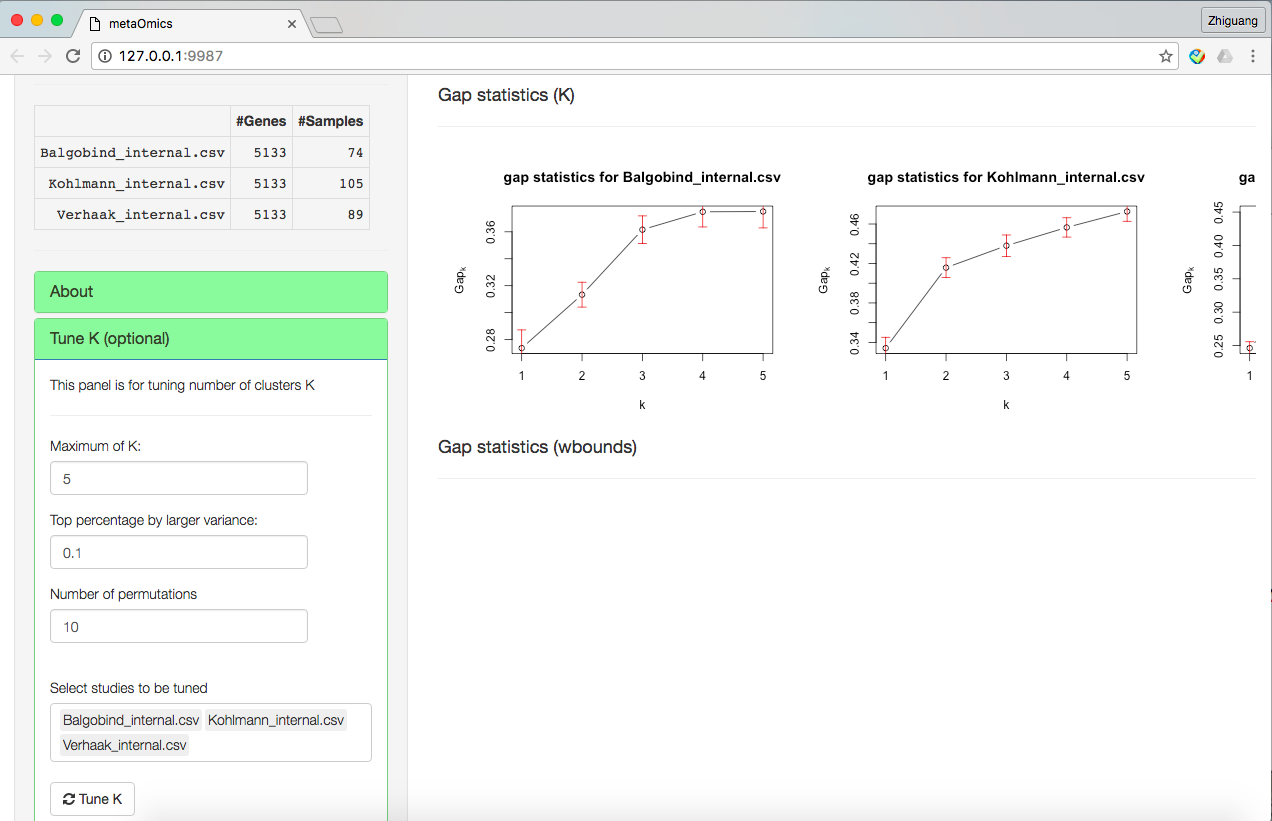
\includegraphics[scale=0.35]{./figure/metaClust/tuneK}
\caption{GUI Preprocessing page}
\label{fig:metaClusttuneK}
\end{center}
\end{figure}
Users will use gap statistics to get optimal K for each individual study.
Users need to specify maximum number of K, which the algorithm will search number of studies from 1 to K.
Top percentage p\% by larger variance means that we will use top p\% larger variance genes to perform gap statistics.
Number of permutation is number of bootstrap samples for gap statistics.
After selecting studies to be tuned and clicking button ``Tune K",
we will obtain gap statistics plat as in Figure~\ref{fig:metaClusttuneK}.
A good K is selected such that the $\mbox{Gap}_k$ is maximized or stablized.
From the figure, K=3 is prefered.


\subsubsection{Tune Wbounds}
Wbounds directly control number of features selected by metaClust.
If the users are not sure what is a good Wbound,
they can start to use the Tune Wbounds panel as in Figure~\ref{fig:metaClusttuneW}.
\begin{figure}[H]
\begin{center}
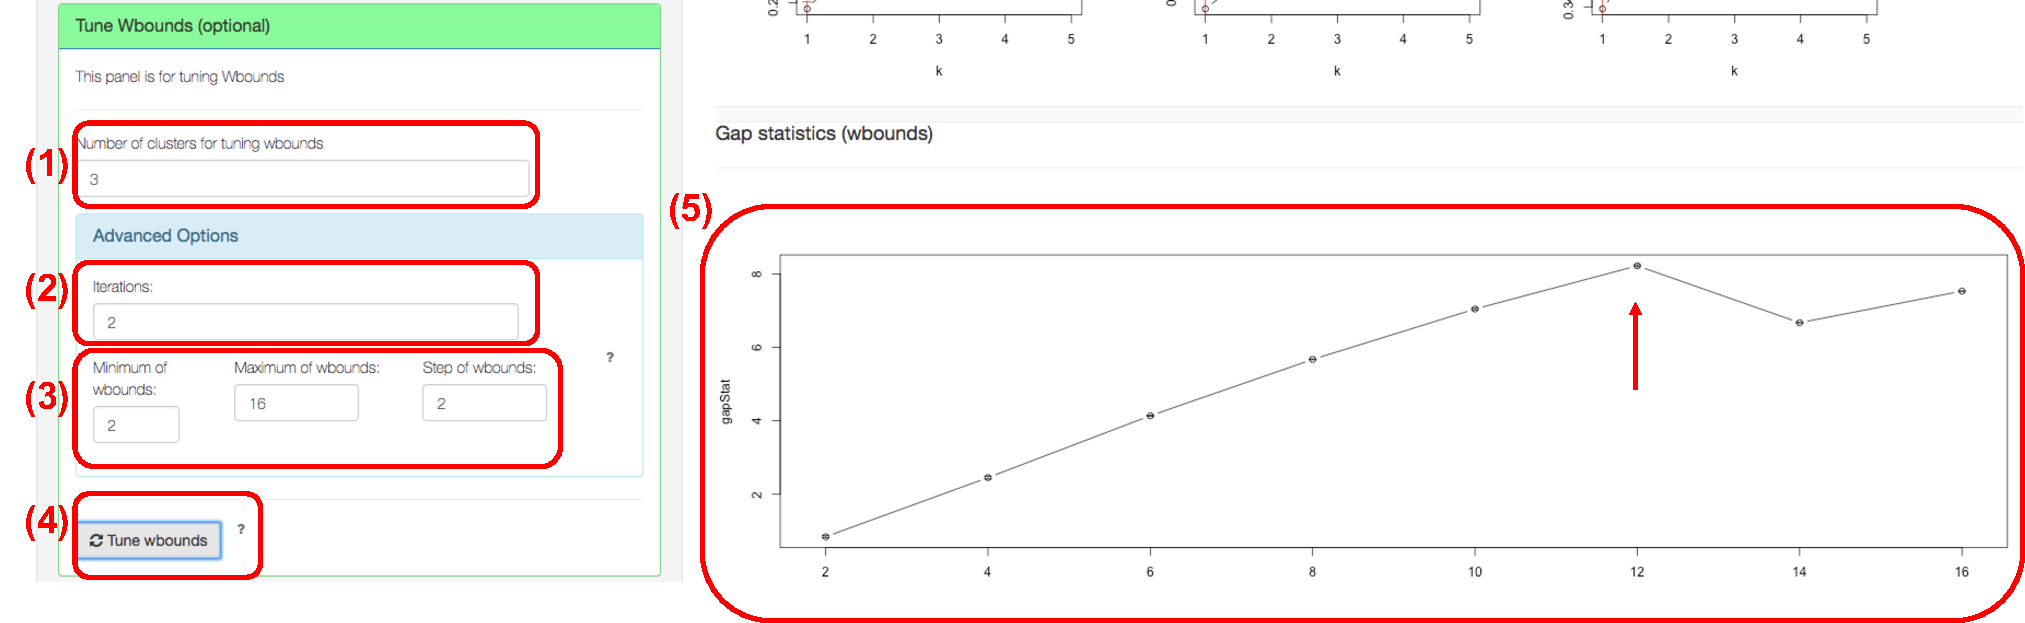
\includegraphics[scale=0.35]{./figure/metaClust/tuneW}
\caption{GUI Preprocessing page}
\label{fig:metaClusttuneW}
\end{center}
\end{figure}
Again,
gap statistics will be used for tuning Wbounds.
Users will specify number of clusters for tuning Wbounds, which could be obtained from the previous step.
Iterations is the same thing as number of bootstrap samples for gap statistics.
Users also need to specify the searching space of Wbounds by minimum of Wbounds, maximum of Wbounds and Step of Wbounds.
After all these steps are set,
user can click on ``Tune Wbounds" button.
The results will be shown in Figure~\ref{fig:metaClusttuneW}.
Wbound=12 is preferred since the corresponding gap statistics is maximized.

\subsubsection{Run Meta Sparse K-Means}
Under Run Meta Sparse K-Means panel,
user can specify number of clusters, Wbounds and run meta sparse K means, 
as in Figure~\ref{fig:mskmRes}.
\begin{figure}[H]
\begin{center}
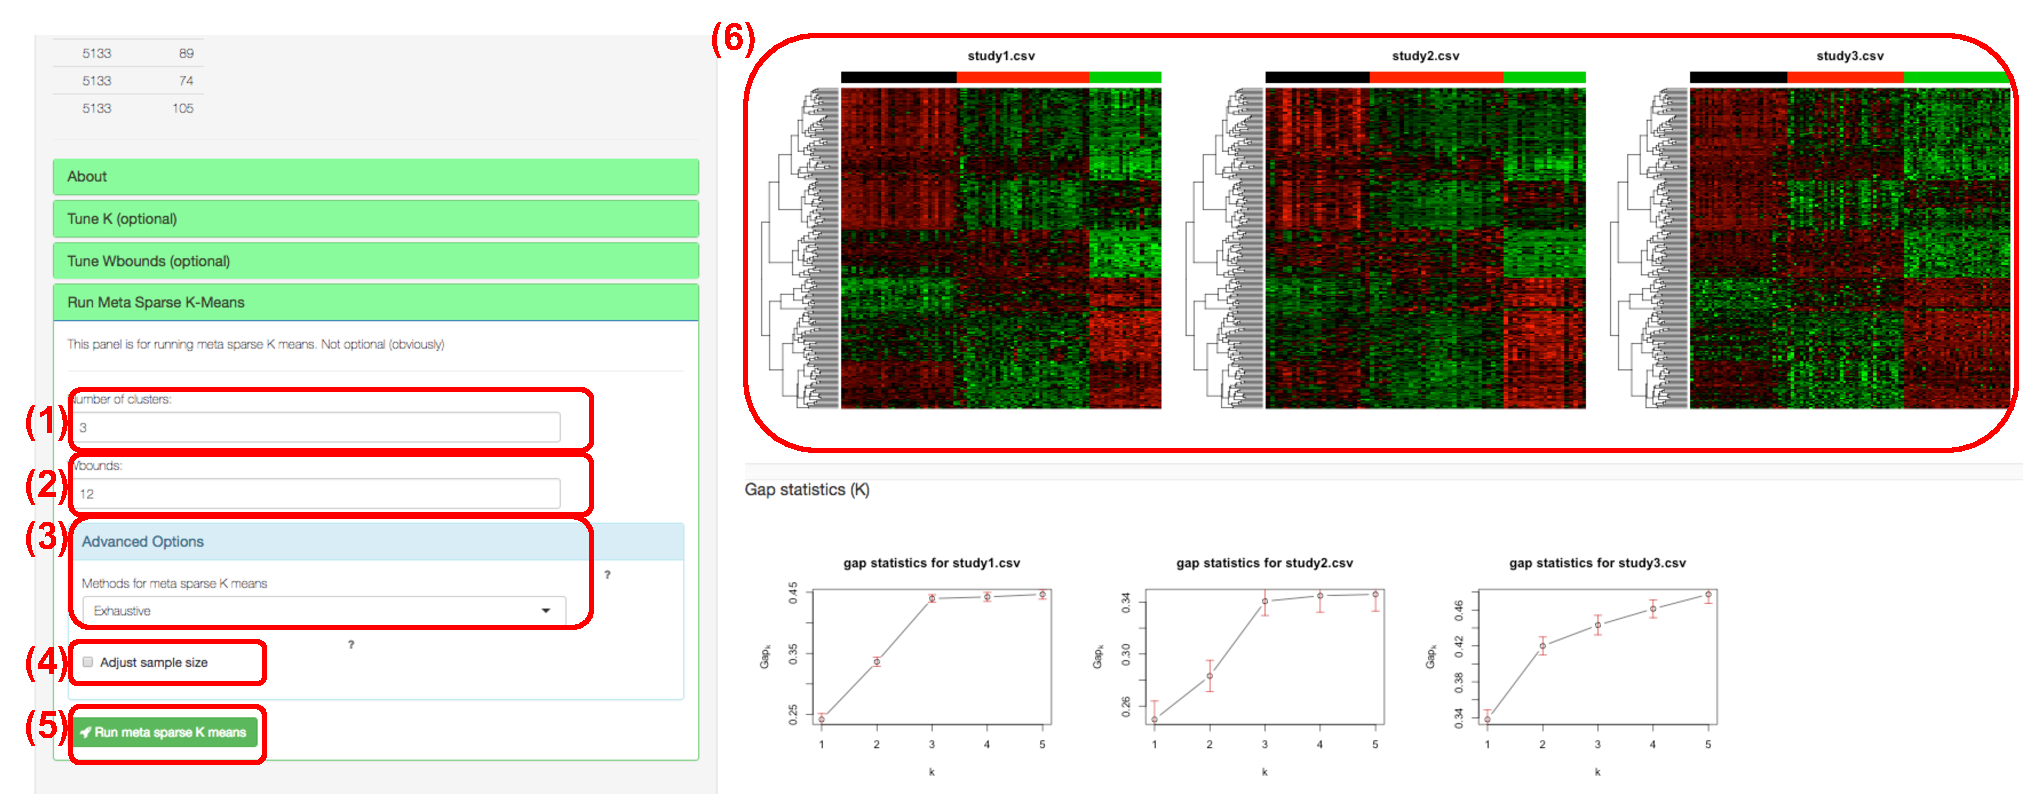
\includegraphics[scale=0.35]{./figure/metaClust/mskmRes}
\caption{GUI Preprocessing page}
\label{fig:mskmRes}
\end{center}
\end{figure}
There are three clustering matching methods: Exhaustive, linear, MCMC.
Exhaustive is suggested if the data is not large.
Linear will perform smart search and get solution much faster than Exhaustive, 
but it may yield less accuracy.
MCMC might by very time consuming.
Adjust sample size checkbox allows users to adjust sample size effect.
After number of clusters and Wbounds are specified,
users can click on Run meta sparse K means and obtain results as Figure~\ref{fig:mskmRes}.

\subsection{MetaPCA}

\subsection{MetaKTSP}

\subsection{MetaDCN}

\subsection{MetaLA}

%%  for citation purpose
\bibliographystyle{apalike}
\bibliography{reference}
 
\end{document}